\documentclass[margin=5mm, tikz]{standalone}
\usepackage[utf8x]{inputenc}
\usepackage{tikz}
\usepackage{siunitx}
\usepackage{physics}
\begin{document}
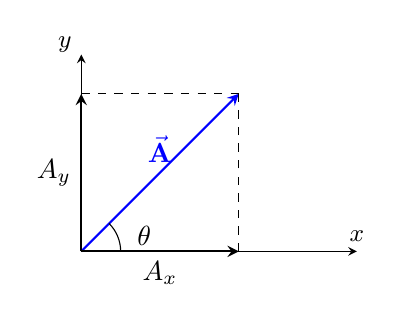
\begin{tikzpicture}
    
    \draw [-stealth] (0, 0) -- (3.5, 0) node [above, pos=1] {\small{$x$}};
    \draw [-stealth] (0, 0) -- (0, 2.5) node [left, pos=1.05] {\small{$y$}};

    \draw [-stealth, thick, color=blue] (0, 0) -- (2, 2) node [above, midway] {$\va{A}$};
    \draw (0.5, 0) arc(0:45:0.5);
    \node at (0.8, 0.2) {$\theta$};
    \draw (0, 0) -- (2.5, 0); 

    \draw [-stealth, thick] (0, 0) -- (0, 2) node [left, midway] {$A_{y}$}; 
    \draw [-stealth, thick] (0, 0) -- (2, 0) node [below, midway] {$A_{x}$};

    \draw [dashed] (0, 2) -- (2, 2);
    \draw [dashed] (2, 0) -- (2, 2);

    
\end{tikzpicture}
\end{document}